\chapter{Объектно-ориентированные модели}

!Почему такое название. Отсылки к MOF и UML. EMF. 
почему Объектно-ориентированные: мы фактически описывает общие правила типизации данных в современных ОО-языках.

!Почему мы используем модели: 
1) это близко к практике в мейнстримовых языках, поскольку модели хорошо отображаются на способы представления информации в ООП. 
2) это достаточно формально, чтобы мы могли строго доказывать свои утверждения.

\section{Синтаксис моделей}

!Мы вводим понятие модели, начиная со структурного представления и постепенно вводя ограничения (аналогично $\lambda$-исчислениям).

\begin{Def}[Модельный терм]
\emph{Модельным термом} называется синтаксическая конструкция, удовлетворяющая следующим правилам:
\[
\begin{array}{rrl}
	\ModelTerm & ::= & \Object{\ModelTerm_{id}}{\ModelTerm_{cl}}{\ModelTerm_{p_1}=\ModelTerm_{v_1},\ldots,\ModelTerm_{p_n}=\ModelTerm_{v_n}}, n \ge 0 \\ 
	           &   | & \Ref{\ModelTerm_{id}} \\ 
	           &   | & \List{MT_1,\ldots,MT_n}, n \ge 0 \\ 
	           &   | & \Set{MT_1,\ldots,MT_n}, n \ge 0 \\ 
	           &   | & \Null \OR \Sigma^* \OR \mathbb{Z} \OR \mathbb{B}, \\
\end{array}
\]
где $\Sigma$ --- некоторый конечный алфавит символов, а $\mathbb{B} = \left\{ \True, \False \right\}$.
\end{Def}

Записывая модельные термы, мы, как правило, не будем заключать строки в кавычки, а будем лишь выделять их шрифтом, чтобы отличать от \emph{метапеременных}: так, $\String{abc}$ --- это строка из трех символов, а $x$ --- метапеременная, которая, в частности может принимать значение $\String{abc}$.

Для различных видом модельных термов мы будем использовать специальные названия. Приведем примеры таких термов и обозначим называния:
\begin{itemize}
\item $\Set{\String{abc}, \Ref{239}, \Null}$ --- \emph{множество}, состоящее из трех констант: строки, числа и специального значения $\Null$;
\item $\List{1, 2, 3}$ --- \emph{список} из трех чисел;
\item $\Object{\String{a}}{\Ref{\String{b}}}{\String{c}=\False}$ --- \emph{объект}, имеющий \emph{идентификатор} $\String{a}$, \emph{ссылку на класс} $\Ref{\String{b}}$ и одно \emph{свойство} $\String{c} = \False$ с идентификатором $\String{c}$ и \emph{значением} $\False$;
\item $\Ref{\String{x}}$ --- \emph{ссылка} на идентификатор $\String{x}$.
\end{itemize}

\emph{Метапеременные} позволяют кратко описать множества термов, обладающих схожей структурой. Так, запись $\Set{a, b}$ описывает все термы-множества, состоящие из двух элементов.

С помощью модельных термов удобно кодировать структуры абстрактного синтаксиса различных языков. В качестве примера приведем такое кодирование для терма $\lambda$-исчисления. Итак, терм $\lambda \, x\,.\,x\,x$ можно представить в виде объекта:
$$
\begin{array}{l}
	\ObjectH{\String{t1}}{\Ref{\String{Abstraction}}}\, \{\\
\indent
	\String{var} = \Object{\String{x}}{\Ref{\String{Variable}}}{\String{name}=\String{x}},\\
\indent
	\String{body} = \ObjectH{\String{t2}}{\Ref{\String{Application}}} \,\{\\
	\indent \indent \String{funciton} = \Object{\String{t3}}{\Ref{\String{Usage}}}{\String{var} = \Ref{\String{x}}}, \\
	\indent \indent \String{argument} = \Object{\String{t4}}{\Ref{\String{Usage}}}{\String{var} = \Ref{\String{x}}} \\
	\indent \}\\
	\}
\end{array}
$$
Из данного представления видно, что объекты модельного терма образуют дерево, соответствующее абстрактному синтаксическому дереву $\lambda$-терма. Обратите внимание на использование ссылок в объектах $\String{t3}$ и $\String{t4}$: значения свойства $\String{var}$ является \emph{ссылкой} на объект, соответствующий определению переменной $\String{x}$. Благодаря ссылкам, дерево объектов можно рассматривать как граф. Наравне с нотацией, введенной выше, мы будем использовать для изображения объектов графическую нотацию, похожую на диаграммы объектов языка \tool{UML} \cite{UML}. На \figref{simplelambda} приведено изображение приведенных выше объектов в виде такой диаграммы.

\begin{figure}[htbp]
\center
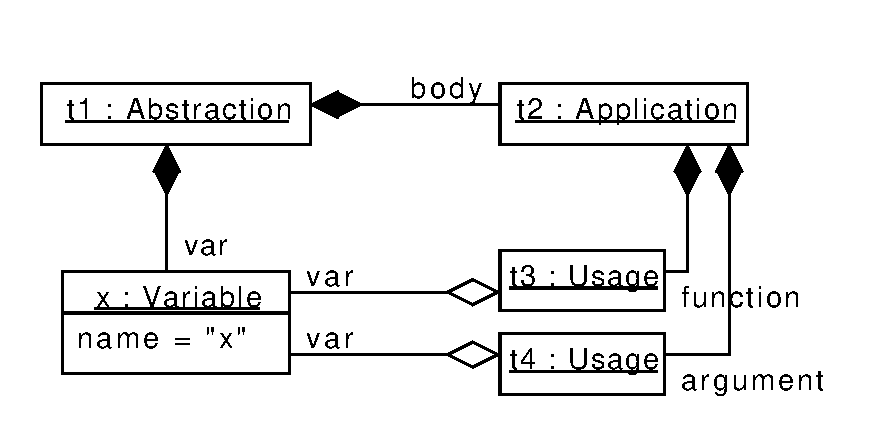
\includegraphics{pictures/simplerlambda.pdf}
\caption{Графическое представление абстрактного синтаксиса для $\lambda$-терма}\label{simplelambda}
\end{figure}

Как видно из рисунка, объекты обозначаются прямоугольниками. В верхней части прямоугольника располагается подчеркнутая надпись: это идентификатор объекта и \emph{имя класса}. О классах мы будем подробно говорить ниже, а пока лишь заметим, что объекты относящиеся к одному классу, должны иметь одинаковую структуру. Значения свойств изображаются либо под горизонтальной чертой в самом прямоугольнике (как для объекта $\String{x}$), либо в виде ребер графа. Ближе к концу ребра написано имя свойства, а в начале ребра изображается ромб: белый, если ребро соответствует ссылке, и черный, если значением свойства является объект, то есть имеет место \emph{агрегация} --- один объект является частью другого. Таким образом, если рассматривать только ребра с черными ромбами, граф объектов превращается в дерево --- то самое, которое соответствует текстовой нотации, введенной выше.

\begin{Def}
Отношение \emph{конгруэнтности} на модельных термах, \mbox{$\MCong \;\subset \ModelTerm \times \ModelTerm$}, есть минимальное отношение эквивалентности, обладающее следующими свойствами:
\begin{enumerate}
\item (Константы) $x \MCong x$, для любого $x \in \left\{\ \Null \right\} \cup \IntegerT \cup \BooleanT \cup \StringT \cup \CharT$;
\item (Ссылки) $\Ref{x} \MCong \Ref{y}$, если $x \MCong y$;
\item (Списки) $\List{x_1, \ldots, x_n} \MCong \List{y_1, \ldots, y_n}$, если $x_i \MCong y_i$ для любого $i \in [1; n]$;
\item (Множества) Если существует перестановка $\pi$ размера $n$ такая, что \mbox{$x_i \MCong x'_{\pi(i)}$} при \mbox{$i \in [1;n]$}, то $\Set{x_1, \ldots, x_n} \MCong \Set{x'_{\pi(1)}, \ldots, x'_{\pi(n)}}$.
\item (Объекты) Аналогично, если $id_1 \MCong id_2$, а также $c_1 \MCong c_2$, и существует перестановка $\pi$ размера $n$ такая, что $p_i \MCong p'_{\pi(i)}$ и $v_i \MCong v'_{\pi(i)}$, то 
$$ 
\Object{id_1}{c_2}{
	\mbox{\small$\begin{array}{c}
		p_1=v_1,\\ 
		\ldots,\\ 
		p_n=v_n
	\end{array}$}
} \MCong \Object{id_2}{c_2}{
	\mbox{\small$\begin{array}{c}
		p'_{\pi(1)}=v'_{\pi(1)},\\
		\ldots,\\
		p'_{\pi(n)}=v'_{\pi(n)}	
	\end{array}$}
};
$$
\end{enumerate}
\end{Def}

Другими словами, термы являются конгруэнтными в случае попарной конгруэнтности соответствующих подтермов, причем при сравнении множеств порядок элементов не важен, а при сравнении объектов не важен порядок свойств. Приведем несколько примеров:
$$
\begin{array}{rcl}
\Ref{abc} \MCong \Ref{abc}
\quad 
\List{1, 2} &\red{\nMCong} & \List{2, 1}
\quad
\Set{1, 2} \MCong \Set{2, 1}
\\
\Object{abc}{\Ref{c}}{\mbox{
\small$\begin{array}{rcl}
a &=& b\\
c &=& d\\
\end{array}$
}} &\MCong & \Object{abc}{\Ref{c}}{\mbox{
\small$\begin{array}{rcl}
\mathbf{c} &=& \mathbf{d}\\
\mathbf{a} &=& \mathbf{b}\\
\end{array}$
}}\\
\Object{abc}{\Ref{c}}{\mbox{
\small$\begin{array}{rcl}
a &=& b\\
c &=& d\\
\end{array}$
}} &\red{\nMCong} & \Object{abc}{\Ref{c}}{\mbox{
\small$\begin{array}{rcl}
c &=& \mathbf{\red{b}}\\
a &=& \mathbf{\red{d}}\\
\end{array}$
}}
\end{array}
$$

Введем функцию $\Objects{t}$, вычисляющую множество всех объектов, являющихся подтермами терма $t$:
$$
	\Objects{t} = \left\{
\begin{array}{ll}
%
\multicolumn{2}{l}{\{t\} \cup \Objects{id} \cup \Objects{c} \cup \bigcup\limits_i \Objects{p_i} \cup \bigcup\limits_i\Objects{v_i},} \\
&          t = \Object{id}{c}{p_1=v_1, \ldots, p_n=v_n}\\
%
\Objects{r},& t = \Ref{r}\\
%
\bigcup\limits_i\Objects{x_i},& t = \List{x_1, \ldots, x_n}\\
%
\bigcup\limits_i\Objects{x_i},& t = \Set{x_1, \ldots, x_n}\\
%
\emptyset, & \mbox{ в остальных случаях}
\end{array}	
	\right.
$$

Аналогично вводятся функция $\Sets{t}$, вычисляющая множество всех множеств-подтермов $t$, и функция $\Refs{t}$, вычисляющая множество всех ссылок-подтермов $t$.

\begin{Def}
Модельный терм $t$ называется \emph{правильно сформированным}, если выполняются следующие условия:
\begin{enumerate}
\item Среди подтермов $t$ не существует двух объектов с конгруэнтными идентификаторами; \label{a}
\item В $\Objects{t}$ не существует объекта, содержащего два свойства с конгруэнтными именами; \label{b}
\item В $\Sets{t}$ не существует множества, содержащего два конгруэнтных элемента. \label{c}
\end{enumerate}
\end{Def}

Так, например, терм $\List{\Object{\red{a}}{\Ref{c}}{}, \Object{\red{a}}{\Ref{c}}{x=y}}$ не является правильно сформированным (пункт \ref{a}). Терм $\Object{a}{\Ref{c}}{\red{a} = b, \red{a} = c}$ тоже не является правильно сформированным, но по другой причине см. пункт \ref{b}. Согласно пункту \ref{c}, терм $\Set{\red{1}, 2, \red{1}}$ также не является корректно сформированным.

\begin{Def}[Ссылочный контекст]
Будем называть \emph{ссылочным контекстом} функцию 
\mbox{$\RContext : \ModelTerm \rightarrow \ModelTerm$}, обладающую следующими свойствами: 
\begin{enumerate}
\item Если $\RContext(id)$ определено, то $\RContext(id) = \left\{\Object{id'}{\ldots}{\ldots}\right\}$, где $id \MCong id'$;
\item $\RContext(id) \MCong \RContext(id')$ тогда и только тогда, когда $id \MCong id'$.
\end{enumerate}
\end{Def}

Другими словами, ссылочный контекст ``находит'' объект по его идентификатору. Для удобства мы будем писать $\RContext(id)=\bot$ в случае, если $\RContext(id)$ не определено.

Обозначим множество всех объектов, \emph{упомянутых} в контексте $\RContext$ (то есть являющихся подтермами элементов области определения $\RContext$ и/или области значений $\RContext$) за $\Objects{\RContext}$. Аналогично вводится множество ссылок $\Refs{\RContext}$.

\begin{Def}\label{RContext}
Будем называть ссылочный контекст $\RContext$ \emph{замкнутым}, если 
$$
	o=\Object{id}{\ldots}{\ldots} \in \Objects{\RContext} \Rightarrow \RContext(id)=o
$$
и
$$
	r=\Ref{id} \in \Refs{\RContext} \Rightarrow \RContext(id) \neq \bot
$$
\end{Def}

Все объекты, упомянутые в замкнутом контексте, могут быть получены по своим идентификаторам, и каждая ссылка ссылается на существующий объект. Из этого, в частности, следует, что в таком контексте каждому объекту присвоен уникальный идентификатор. Так, например, следующий контекст является замкнутым:
\begin{equation*}
	\RContext(id) = \left\{
		a \mapsto \Object{a}{\Ref{a}}{} \right\}
\end{equation*}
Приведем также пример незамкнутого контекста:
\begin{equation*}
	\RContext(id) = \left\{
		a  \mapsto  \Object{a}{\red{\Ref{b}}}{c = \red{\Object{b}{\Ref{a}}{}}}
\right\}
\end{equation*}
в последнем примере нарушаются оба требования определения \ref{RContext}: 
\begin{itemize}
\item объект, упомянутый в контексте, не принадлежит области его значений;
\item ссылка, упомянутая в контексте, не принадлежит его области определения.
\end{itemize}

\begin{Def}
Пусть $\RContext_1$ и $\RContext_2$ -- ссылочные контексты с непересекающимися областями определения ($\forall x \in D(\RContext_1), y \in D(\RContext_2): x \nMCong y$). Тогда их \emph{объединение} определяется следующей формулой:
$$
	\left(\RContext_1 \cup \RContext_2\right)(id) = \left\{
	\begin{array}{ll}
		\RContext_1(id), & \RContext_1(id) \neq \bot \\
		\RContext_2(id), & \RContext_2(id) \neq \bot \\
		\bot,            & \mbox{в противном случае.}
	\end{array}
	\right.
$$
\end{Def}

По модельному терму $t$ можно построить ссылочный контекст, упоминающий все объекты, входящие в $t$:
$$
	\RContext_t = \left\{ id \mapsto o \;|\; o = \Object{id}{\ldots}{\ldots} \in \Objects{t}\right\}
$$

\begin{Def}[Пред-модель]
Будем называть правильно сформированный модельный терм $t$ \emph{пред-моделью в контексте $\RContext_0$}, если контекст $\RContext_0 \cup \RContext_t$ является замкнутым.
\end{Def}

Пред-модель обладает важным свойством: любой объект в ней однозначно определяется своим идентификатором, и любая ссылка указывает на известный объект.

\section{Классы и типы}

!На практике для удобства навигации по моделям и контроля над их корректностью вводятся дополнительные ограничения (в виде системы типов), регулирующие структуру моделей. Сами эти ограничения также записываются в виде моделей...

\begin{Def}[Класс]
\emph{Классом} называется кортеж $\langle id, S, P \rangle$, где 
\begin{enumerate}
\item $id$ --- \emph{идентификатор} класса,
\item $S$ --- множество классов, называемых \emph{предками} данного класса (\emph{суперклассов}),
\item $P$ --- множество пар вида $p : \tau$, где $p$ --- \emph{идентификатор} свойства, а $\tau$ --- \emph{тип} свойства (множество типов определяется ниже).
\end{enumerate}
Множество $P$ не содержит различных пар, в которых совпадают идентификаторы свойств.
\end{Def}

Для удобства, мы будем обозначать класс $\langle id, S, P \rangle$ через \mbox{$\Class{id}{S}{P}$}. 

\begin{Def}
Множество типов $\Types$ описывается следующим образом:
$$
\begin{array}{rrl}
\Types &::=& \CharT \OR \StringT \OR \IntegerT \OR \BooleanT \\
         &|& \NullableT{\Types} 
         \OR \SetT{\Types^+} \OR \SetT{\Types^*}
         \OR \ListT{\Types^+} \OR \ListT{\Types^*}\\
         &|& \ClassT{c} \OR \RefT{c}, \mbox{ где $c$ --- идентификатор некторого класса} \\
         &|& \AnyT \\
\end{array}
$$
\end{Def}
\noindent Поясним интуитивное значение данного определения:
\begin{itemize}
\item $\CharT$, $\StringT$, $\IntegerT$, $\BooleanT$ обозначают примитивные типы: символы, строки, целые числа и булевские значения соответственно.
\item Тип $\NullableT{\tau}$ допускает значение $\Null$ или значение типа $\tau$, например, $\NullableT{\CharT}$ соответствует множеству значений $\Sigma \cup \{\Null\}$.
\item $\SetT{\tau^*}$ обозначает тип множеств, содержащих ноль или более элементов типа $\tau$. Например, $\SetT{\StringT^*}$ --- 
это множества строк, а $\SetT{\Set{\IntegerT^*}^*}$ --- множества множеств целых чисел. 
\item Аналогично, $\ListT{\tau^*}$ обозначает списки. 
\item Если вместо ``*'' используется ``+'', то множество или список должны содержать не менее одного элемента. Например, $\SetT{\tau^+}$ --- непустые множества, составленные из элементов $\tau$. 
\item $\ClassT{c}$, где $c$ --- некоторый класс (точнее, его идентификатор), соответствует \emph{агрегированному} объекту класса $c$. В качестве примера терм $\Object{a}{\Ref{c}}{a = \Object{b}{\Ref{c}}{}}$: здесь объект $b$ содержится внутри объекта $a$, такая ситуация и называется \emph{агрегированием}.
\item $\RefT{c}$ обозначает тип ссылок на объекты класса $c$, то есть значений вида $\Ref{a}$, где $a$ --- идентификатор объекта, принадлежащего к классу $c$ (см. ниже).
\item $\AnyT$ (``Top'') --- супертип всех остальных типов (см. ниже).
\end{itemize}

Для типа $\tau$, множество упомянутых в данном типе классов определяется следующим образом:
$$
	\Classes{\tau} = \left\{
	\begin{array}{ll}
		\{c\}, & \tau \in \left\{\ClassT{c}, \RefT{c}\right\}\\
		\Classes{\sigma}, & \tau \in \left\{\ListT{\sigma^+}, \ListT{\sigma^*}, \SetT{\sigma^+}, \SetT{\sigma^*}, \NullableT{\sigma}\right\}\\
		\emptyset, & \mbox{в остальных случаях}\\
	\end{array}
	\right.
$$

Пусть дано множество классов 
$$
C = \{\Class{id_i}{S_i}{p^i_j : \tau^i_j \OR j \in [1;m_i]}\OR i \in [1;n]\},
$$
обозначим $\AllSuperclasses{C} = C \cup \AllSuperclasses{\bigcup_1^n S_i}$ множество всех классов из $C$, их предков, предков их предков и т.д.

Аналогично определяется множество всех свойств класса $c = \Class{id}{S}{p_i : \tau_i}$. Кроме свойств $p_i$, объявленных в самом $c$, рассматриваются также свойства, \emph{унаследованные} из суперклассов:  $\AllProps{C} = \bigcup\limits_{i = 1}^n\{p^i_j : \tau^i_j \OR j \in [1;m_i]\} \cup \AllProps{\AllSuperclasses{C}}$.

\begin{Def}
Конечный набор классов $C$ называется \emph{корректным}, если выполняются следующие свойства:
\begin{enumerate}
\item Все предки классов из $C$ содержатся в $C$: $\AllSuperclasses{C} = C$.
\item Все типы свойств классов из $C$ упоминают только классы из $C$: пусть $\AllProps{C} = \left\{p_i : \tau_i\right\}$, тогда $\bigcup_i \Classes{\tau_i} \subseteq C$.
\item Никакой класс из $C$ не является прямым или непрямым предком самого себя: если $c = \Class{id}{S}{\ldots} \in C$, то $c \notin \AllSuperclasses{S}$.
\end{enumerate}
\end{Def}

На типах, порожденных корректным набором классов $C$, вводится отношение ``подтип'' ($\subtype$) --- это наименьшее транзитивное рефлексивное отношение, обладающее следующими свойствами:
$$
\infer[subclass]{
\type{\mbox{TO}}{c} \subtype \type{\mbox{TO}}{s}
}{
	\Class{c}{S}{\ldots} \in C &
	s \in S & 
	\mbox{TO} \in \{\valts,\, \refts\}
}
$$  $$
\infer[option]{
	\tau \subtype \NullableT{\tau}
}{}
\quad
\infer[multiplicity]{
+ < *
}{}
$$ $$
\infer[set]{
	\SetT{\tau^\iota} \subtype \SetT{\sigma^\kappa}
}{
	\tau \subtype \sigma &
	\iota, \kappa \in \{+, *\} &
	\iota \le \kappa
}
\quad
\infer[list]{
	\ListT{\tau^\iota} \subtype \ListT{\sigma^\kappa}
}{
	\tau \subtype \sigma &
	\iota, \kappa \in \{+, *\} &
	\iota \le \kappa
}
$$

Классы и типы используются для описания допустимых конфигураций модельных термов. Пусть зафиксирован замкнутый ссылочный контекст $\RContext$. Введем функцию $\semRC{\bullet} : \Types \rightarrow 2^{\ModelTerm}$, которая возвращает все модельные термы, упомянутые в контексте $\RContext$, принадлежащие к данному типу. Эта функция задается следующим образом. Типу $\ClassT{c}$ ставится в соответствие множество $\semRC{\ClassT{c}}$ всех объектов из $\Objects{\RContext}$, имеющих ссылкой на класс $\Ref{c}$ и имеющих все свойства из множества $\AllProps{c}$ и только их, причем значение каждого свойства имеет тип, указанный для данного свойства в классе:
$$
\infer[objects]{
	\semRC{\ClassT{c}} = \left\{
		\Object{id}{\Ref{c}}{p_i = v_i} \in \Objects{\RContext}
		\,|\,
		v_i \in \semRC{\tau_i} 
	\right\}
}{
	\Class{c}{S}{\ldots}&
	\AllProps{c} = \left\{p_1 : \tau_1, \ldots, p_n : \tau_n\right\}
}
$$ 
Другие типы характеризуются следующим образом:
$$
\infer[refs]{
	\semRC{\RefT{c}} = \left\{ \Ref{id} \in \Refs{\RContext} \,|\, \RContext(id) \in \semRC{\ClassT{c}} \right\}
}{
	\Class{c}{S}{\ldots}
}
$$ $$
\infer[set]{
	\semRC{\SetT{\tau^+}} = \left\{ \Set{x_1,\ldots,x_n} \,|\, x_i \in \semRC{\tau}\right\}
}{
}
$$ $$
\infer[list]{
	\semRC{\ListT{\tau^+}} = \left\{ \List{x_1,\ldots,x_n} \,|\, x_i \in \semRC{\tau}\right\}
}{
}
$$ $$
\infer[eset]{
	\semRC{\SetT{\tau^*}} = \semRC{\SetT{\tau^+}} \cup \left\{ \Set{} \right\}
}{}	
\quad
\infer[elist]{
	\semRC{\ListT{\tau^*}} = \semRC{\ListT{\tau^+}} \cup \left\{ \List{} \right\}
}{}	
$$ $$
\infer[null]{
	\semRC{\NullableT{\tau}} = \semRC{\tau} \cup \{\Null\}
}{
}
\quad
\infer[primitive]{
	\sem{\Types_P} = \Types_P
}{
	\Types_P \in \{\IntegerT, \CharT, \StringT, \BooleanT\}
}
\quad
$$

Определение функции $\semRC{\bullet}$ не согласуется с отношением $\subtype$: отношение наследования (предок-потомок) на классах не отражено во вложенности множеств, соответствующих типам. Чтобы устранить этот недостаток, введем для корректного набора классов $C$ функцию $\denotRCC{\bullet}$, определяемую следующим образом:
$$
\begin{array}{rcl}
	\denotRCC{\tau} &=& \semRC{\tau} \cup \bigcup_{\sigma \subtype \tau} \semRC{\sigma}\\
	\denotRCC{\top} &=& \bigcup\limits_\tau \semRC{\tau}\\
\end{array}	
$$

\section{Модели и мета-модели}

  @Class PropertyDescriptor {
    @Class.abstract = false,
    @Class.superclasses = {},
    @Class.propertyDescriptors = {
      @PropertyDescriptor PropertyDescriptor.type {
        @PropertyDescriptor.type = @ObjectType { @ClassType.class = @Type }
      }
    }
  },
$$
\Object{PropertyDescriptor}{\Ref{Class}}{\mbox{
%\begin{itemize}
%\item[] $\Ref{Class.abstract} = \False$,
%\item[] $\Ref{Class.superclasses} = \Set{}$,
%\item[] $    \Ref{Class.propertyDescriptors} = \Set{
%      \Object{PropertyDescriptor.type}{\Ref{PropertyDescriptor}}{
%        \Ref{PropertyDescriptor.type} = \Object{\_}{ObjectType}{ %\Ref{ClassType.class} = \Ref{Type} }
%      }
%    }$
%\end{itemize}
}}
$$

!Определяя типы, мы использовали идентификаторы классов внутри модельных термов. Чтобы это было возможно, необходимо, чтобы сами классы были модельными термами.

!Мета-модель накладывает ограничения на структуру объектов через типы и кратность ссылок и атрибутов. Эти ограничения мы записываем в виде системы типов, которая связывает мета-модель и объект отношением $\Vdash$. Запись $\fromMM x : \tau$ следует читать как ``\term{объект $x$ удовлетворяет ограничениям мета-модели $\MM{M}$ и имеет тип $\tau$}''.

!Enums!!!!

\begin{figure}[htbp]
	\centering
$$
	\infer[object]{
		\fromMM \Object{id}{\Ref{c}}{p_i = v_i} : \ClassT{c}
	}{
		\Class{c}{S}{P} \in \MM{M}&
		\AllProps{c} = \{p_i : \tau_i\}&
		\fromMM v_i : \tau_i
	}
$$
$$
\infer[ref]{
	\fromMM \Ref{id} : \RefT{c}
}{
	\fromMM \RContext(id) : \ClassT{c}
}
\quad
\infer[null]{
	\fromMM \Null : \NullableT{\tau}
}{}
$$
$$
\infer[elist]{
	\fromMM \List{\,} : \ListT{\tau^*}
}{}
\quad
\infer[list]{
	\fromMM \List{x_1, \ldots, x_n} : \List{\tau^+}
}{
	\fromMM x_i : \tau & \forall i\in[1:n]
}
$$
$$
\infer[eset]{
	\fromMM \Set{\,} : \SetT{\tau^*}
}{}
\quad
\infer[set]{
	\fromMM \Set{x_1, \ldots, x_n} : \SetT{\tau^+}
}{
	\fromMM x_i : \tau & \forall i\in[1:n]
}
$$
$$
\infer[subtype]{
	\fromMM x : \sigma
}{
	\fromMM x : \tau &
	\tau \subtype \sigma
}
$$
$$
\infer[enum]{
	\forall i \in [1:n]. \; \fromMM T.L_i : T
}{
	\mathbf{enum}\;T\{L_1,\ldots,L_n\} \in \MM{M}
}
\quad
\infer[primitive]{
	\fromMM x : \Types_P
}{
	x \in \Types_P & 
	\Types_P \in \{\IntegerT, \CharT, \StringT, \BooleanT\}
}
$$
	\caption{Структурная корректность объектов}\label{TypesMM}
\end{figure}


